\documentclass[../Article_Model_Parameters.tex]{subfiles}
\graphicspath{{\subfix{../Figures/}}}
\begin{document}
	
	\label{CH: Results}

    The parameter estimation problem was solved by fitting the process model to the dataset given in the table \ref{tab: Yield_data}. Each time-series was fitted to the model separately. As a result of fitting, the following parameters were obtained:

    \begin{itemize}
        \item Partition coefficient:\qquad\quad\qquad$k_m$
        \item Internal Diffusion coefficient: \quad$D_i$
        \item Axial Diffusion coefficient: \qquad$D_e^M$
        \item Standard Deviation: \qquad\qquad\quad$\sigma$
    \end{itemize}

    Moreover, the initial state estimation was performed together with parameter estimation. The concentration of solute in the solid phase is assumed to be constant and uniformly distributed. On the other hand, the solute concentration in the fluid phase should not follow the same assumption as the solid phase. During the preparation period the solute diffuses to the fluid phase in contact with the solid particles. Later, the solute in the fluid phase is partially moved (if the pressure increase in the system, the pump cause the movement of the fluid, even if the outlet valve is closed) along the extractor. As a result, the distribution of solutes mass in the fluid phase is assumed to not be uniform. Some conclusions can be drawn from the analysis of the initial part of each yield curve. It can be noticed that each curve at the beginning has a curvature, which is not linear. In a general sense, it can be said that a quadratic function could approximate the initial part of each extraction curve. A function that, after integration, gives a quadratic-like result is a straight line. Based on that observation, the solute concentration in the fluid phase is assumed to be linearly distributed. The solute concentration is assumed to be zero at the outlet and reach the maximum at the beginning of the fixed bed. The details on the calculation are given in appendix \ref{CH: IC_BC}. The linear distribution can be defined if the total mass of solute $m_{total}$ and partition coefficient $\tau$ are know.
    
    Due to initial state estimation, two additional parameters are fitted.

    \begin{itemize}
        \item Total mass of solute: \qquad\qquad\quad$m_{total}$
        \item Partition coefficient: \qquad\qquad\quad$\tau$
    \end{itemize}

	To ensure that parameters found by the optimizer do not reach unrealistic values, an additional set of inequality constraints is introduced. The lower and upper bounds for each parameter are given in Table \ref{tab:Constraints}.

	\begin{table}[!h]
		\begin{tabular}{ l|cccccc } 
			Parameter	&$k_m$ 	& $D_i$ 	& $D_e^M$ 	& $m_{total}$	& $\tau$ 	& $\sigma$ \\  \hline
			Lower bound	&0	  	& 0 	  	& 0 		& 76 		 	& 0 	   	& 0 \\ 
			Upper bound	&1 		& $+\infty$ & $+\infty$	& 100 			& 1 		& $+\infty$ \\
		\end{tabular}
	\caption{Constraints of the parameter estimation problem}
	\label{tab:Constraints}
	\end{table}

	The parameter estimation problem requires an initial guess as an input to an optimization problem. To ensure that the solution is a global solution multiple initial points have been tested. The initial guesses for the parameter estimation problem are given in Table \ref{tab:InitialGuess}
	
	\begin{table}[!h]
		\begin{tabular}{ l|cccccc } 
			Parameter		&$k_m$ 	& $D_i$ 	& $D_e^M$ 	& $m_{total}$	& $\tau$ 	& $\sigma$ \\  \hline
			Initial guess	&1	  	& 3 	  	& 1 		& 77 		 	& 0.65 	   	& 0.1 \\  
		\end{tabular}
		\caption{Constraints of the parameter estimation problem}
		\label{tab:InitialGuess}
	\end{table}

	The results of the parameter estimation can be found in Table \ref{tab: Estimation_results}.
		
	\begin{table}[!h]
		\centering
		\adjustbox{max width=\columnwidth}{%
			\csvautotabular{Figures/Results_estimation/estimation.csv} }
		\caption{Parameter estimation results}
		\label{tab: Estimation_results}
	\end{table}
	
	The figure \ref{fig: estimation_results} show yield plots for each of experiments. The blue dot indicate the data point obtained as a measurement from the laboratory experiments. The black curve represents the yield curve obtained from the initial guess of the parameters. The blue curve correspond to yield curve obtained as a solution of the optimization problem.

	\begin{figure*}[!h]
		\centering
		\begin{subfigure}[b]{0.8\textwidth}
			\centering
			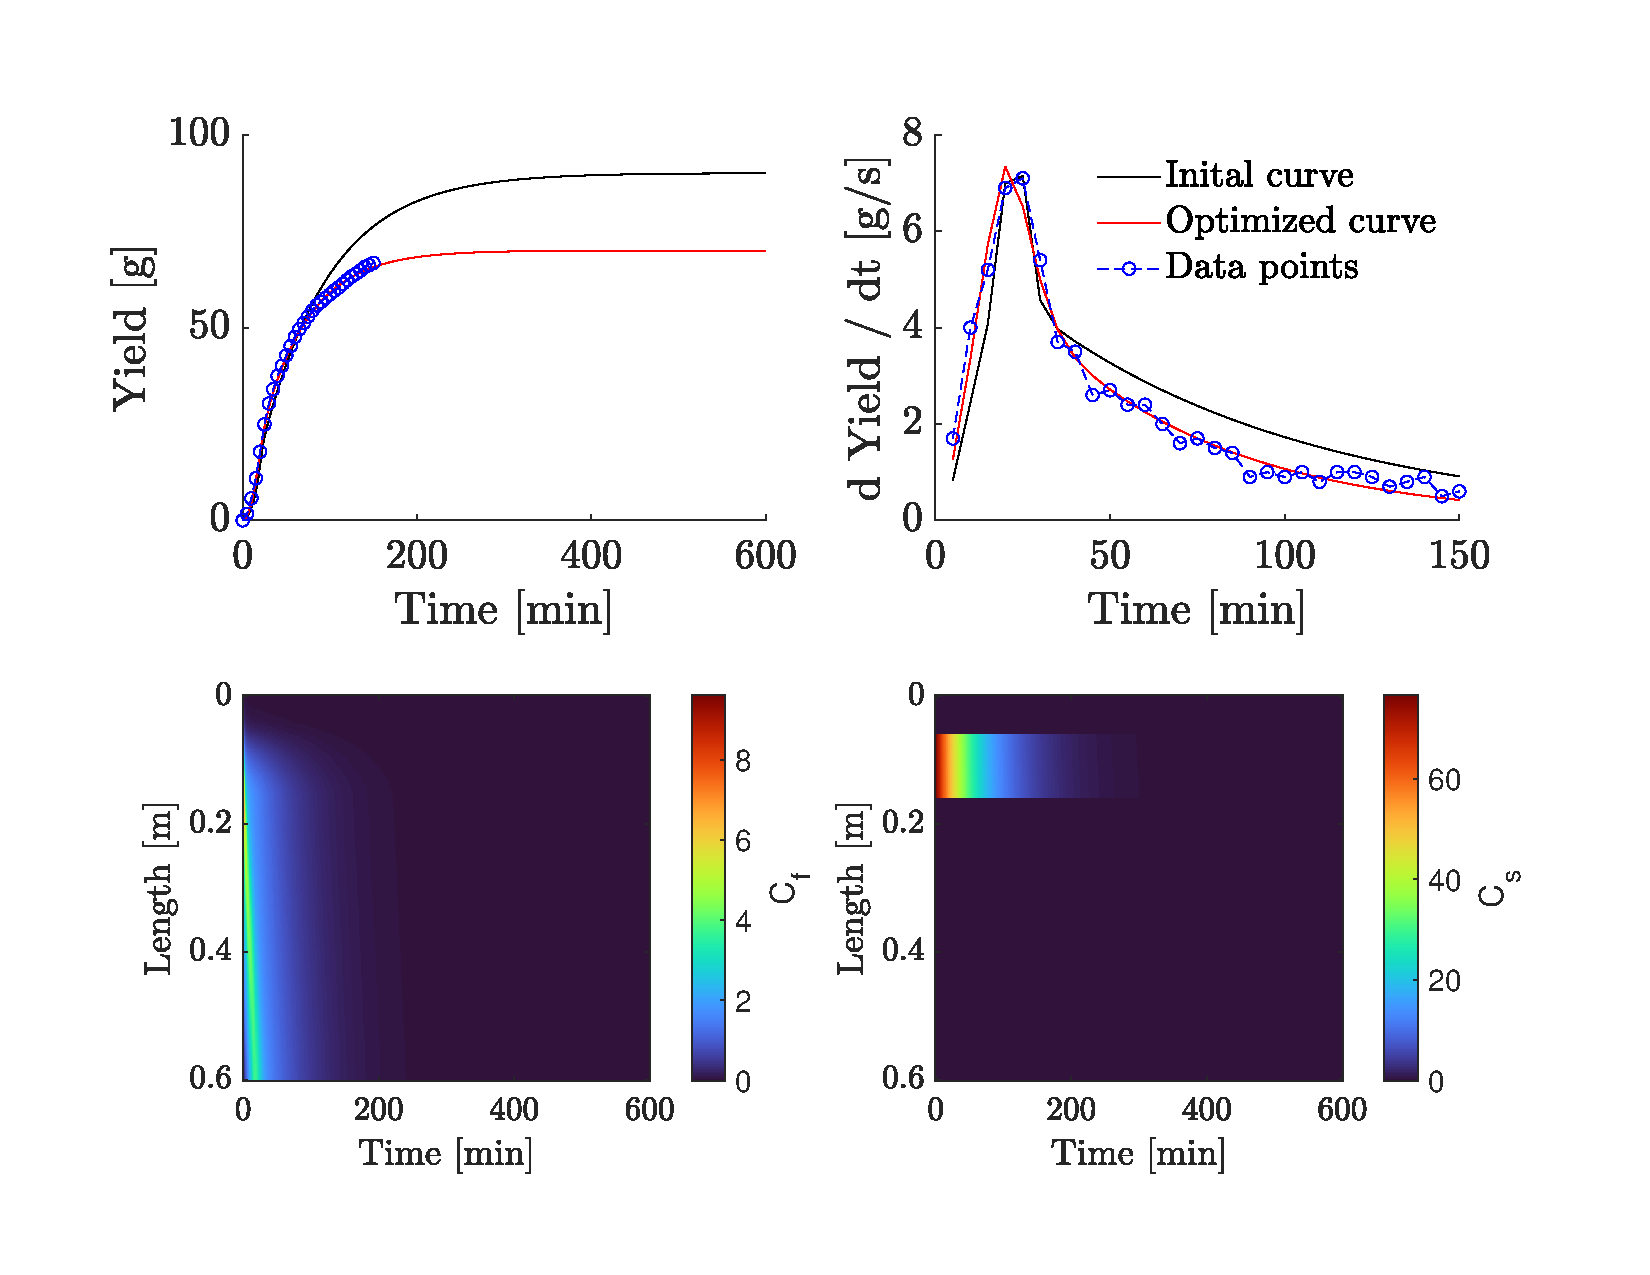
\includegraphics[trim = 3cm 11cm 2.5cm 2.1cm,clip,width=\textwidth]{/Results_estimation/Fitting_LUKE_T40_P200.pdf}
			\caption{Experiment at $40^\circ C$ and $200$ bar}
		\end{subfigure}
		\hfill
		\begin{subfigure}[b]{0.8\textwidth}
			\centering
			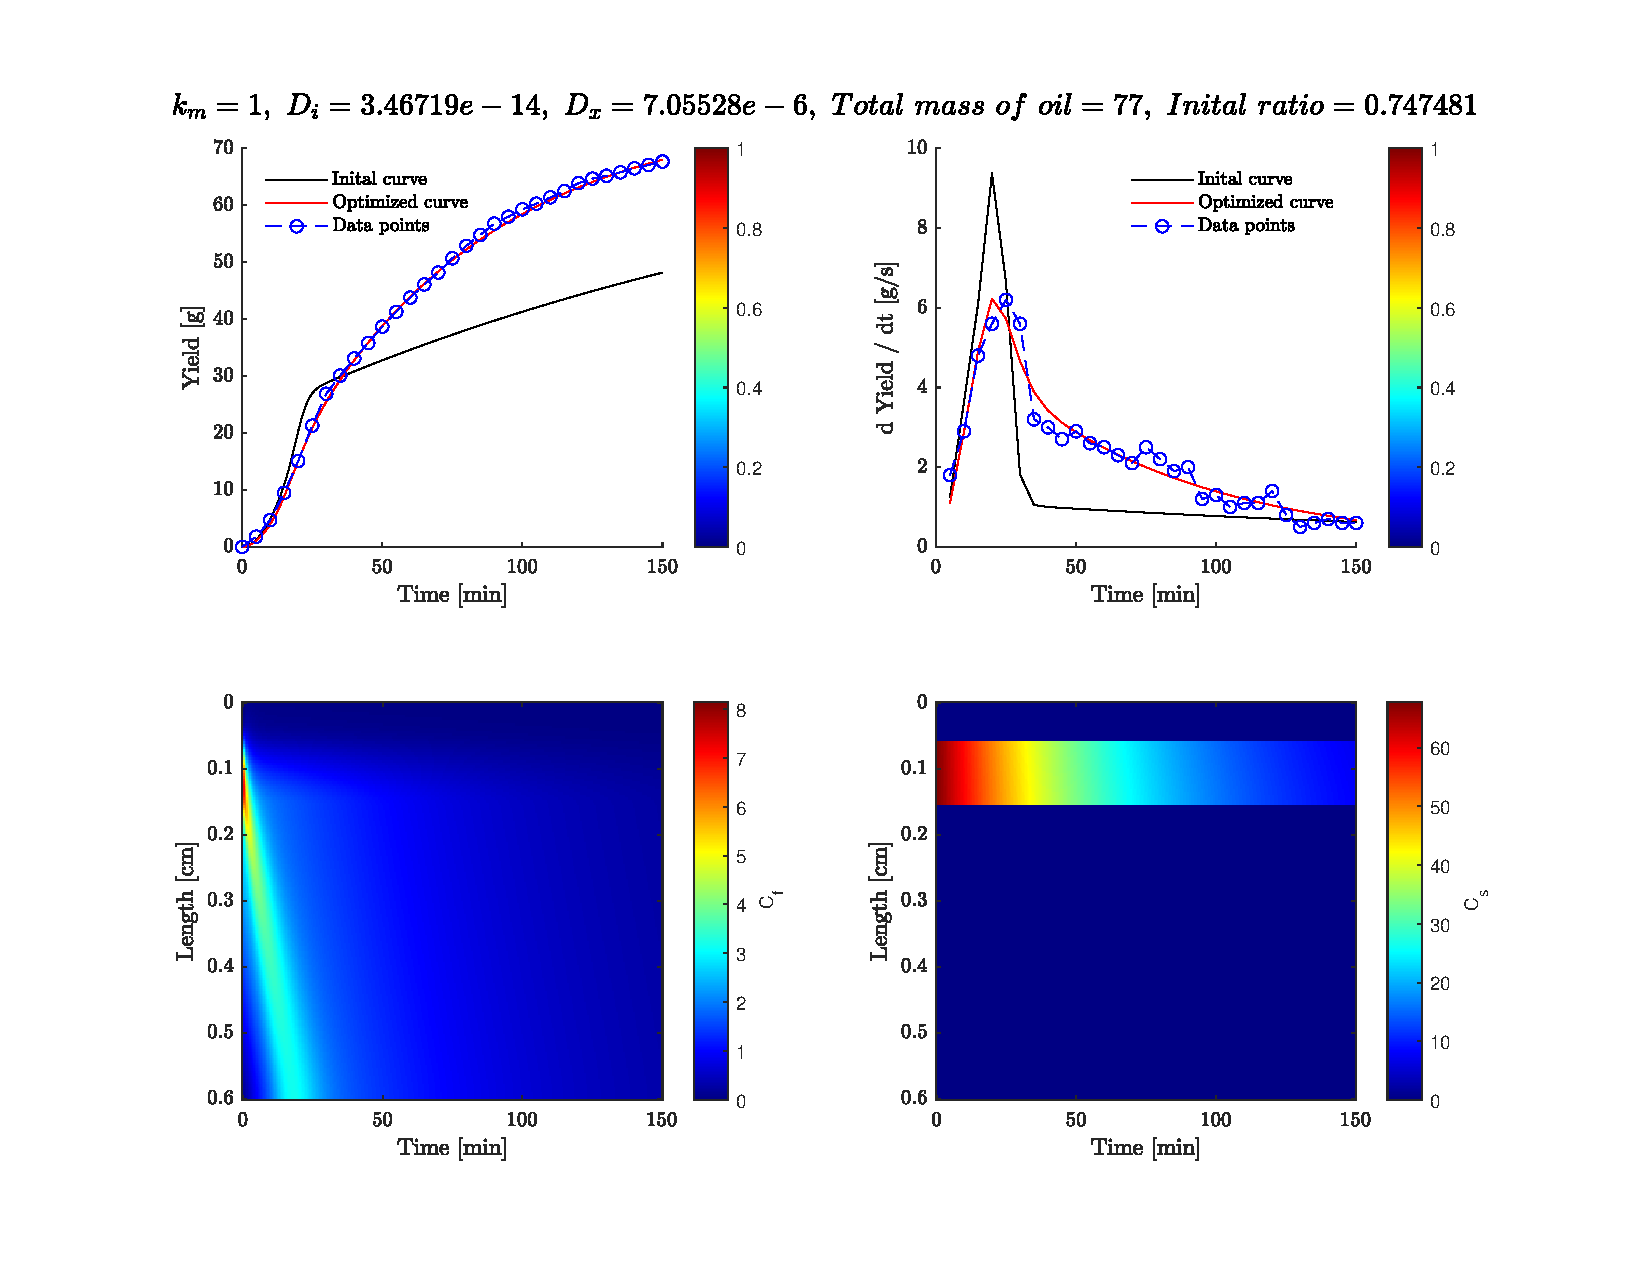
\includegraphics[trim = 3cm 11cm 2.5cm 2.1cm,clip,width=\textwidth]{/Results_estimation/Fitting_LUKE_T50_P200.pdf}
			\caption{Experiment at $50^\circ C$ and $200$ bar}
		\end{subfigure}
		\hfill
		\begin{subfigure}[b]{0.8\textwidth}
			\centering
			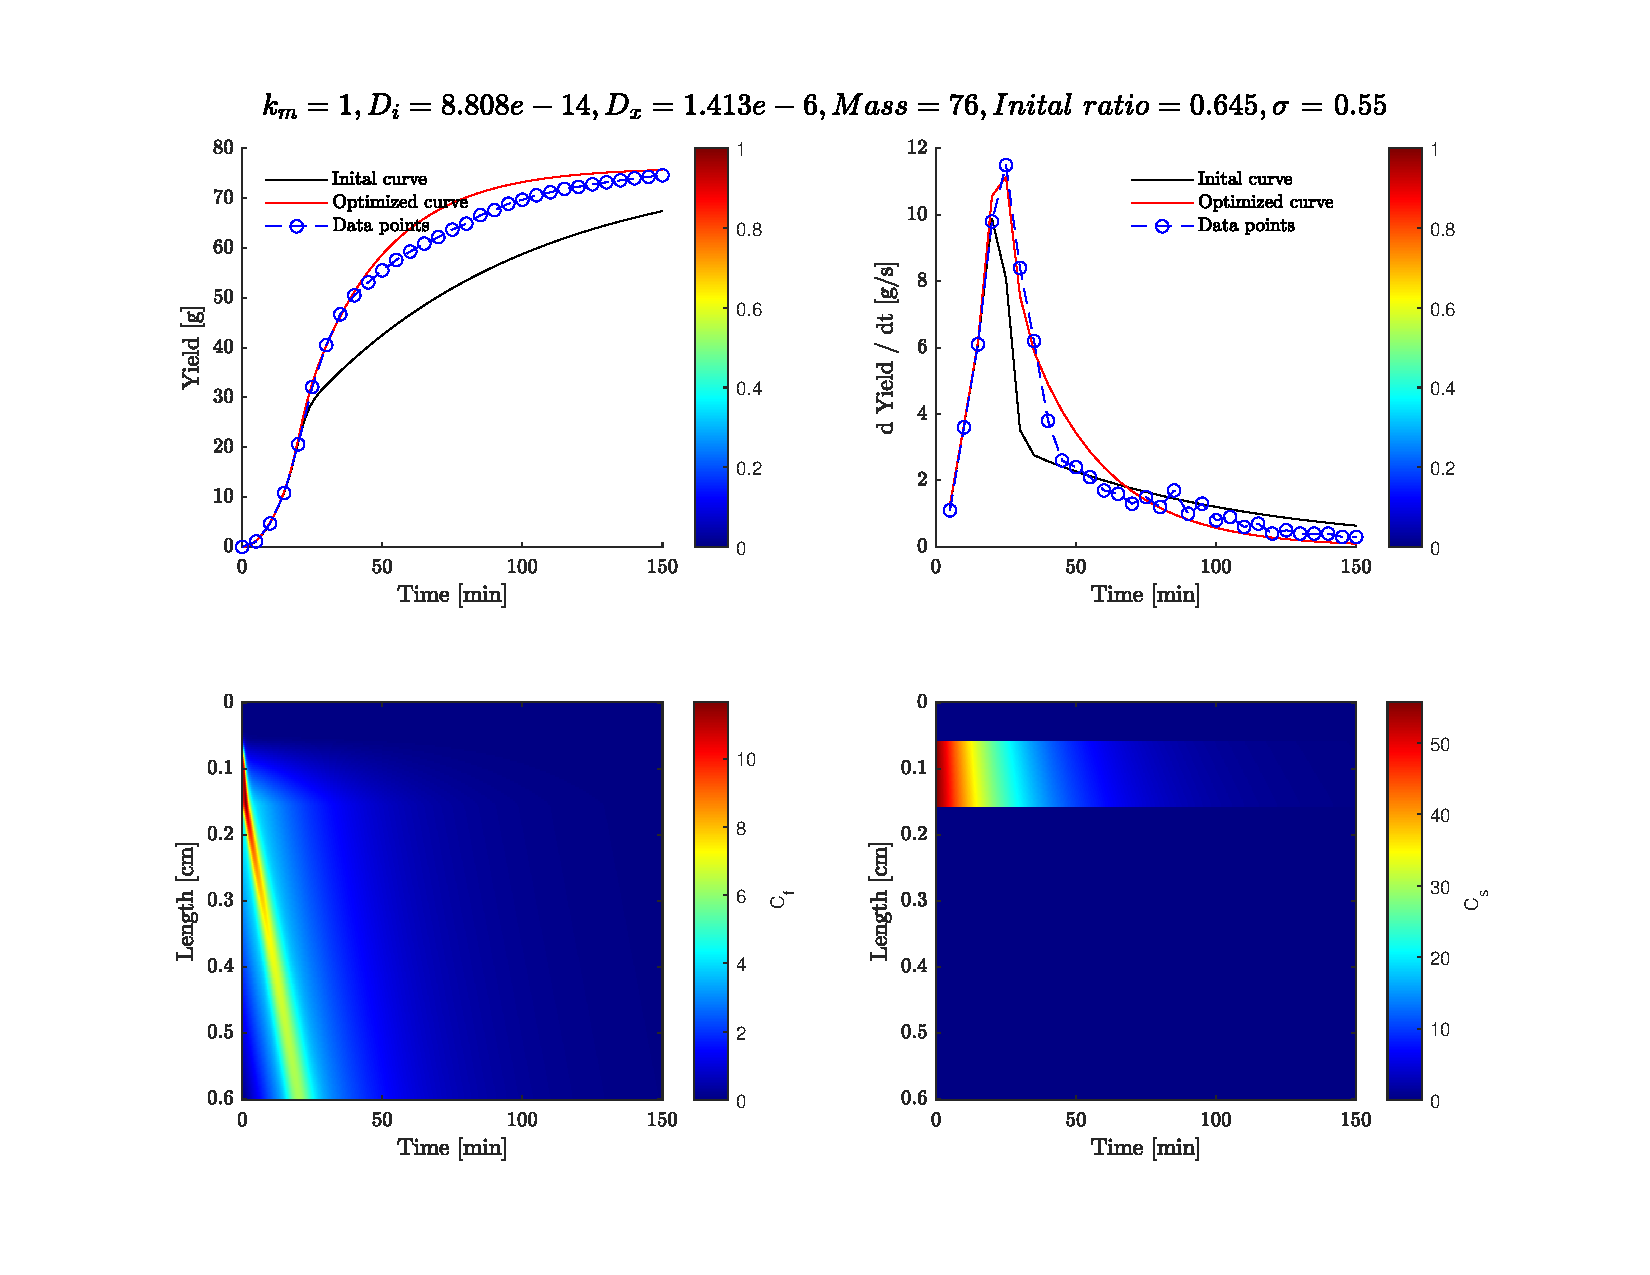
\includegraphics[trim = 3cm 11cm 2.5cm 2.1cm,clip,width=\textwidth]{/Results_estimation/Fitting_LUKE_T40_P300_org.pdf}
			\caption{Experiment at $40^\circ C$ and $300$ bar}
		\end{subfigure}
		\hfill
		\begin{subfigure}[b]{0.8\textwidth}
			\centering
			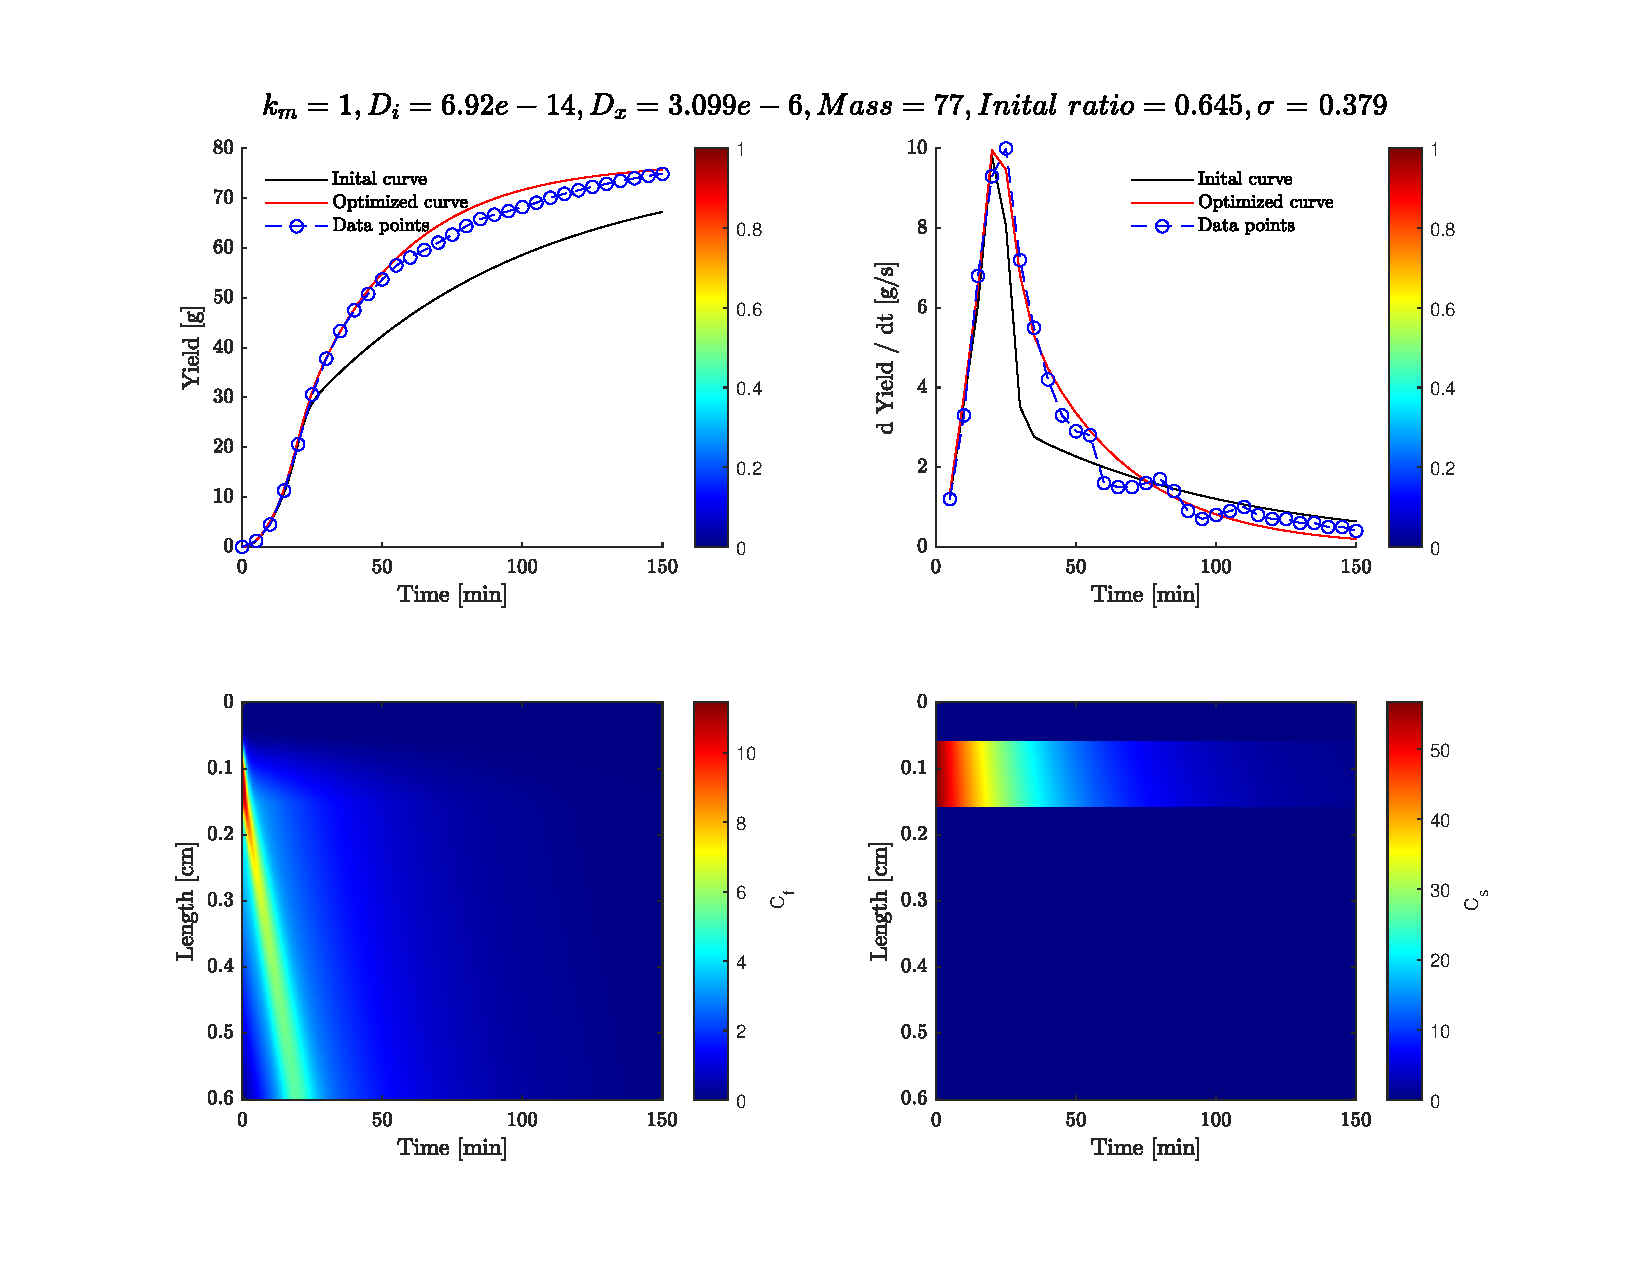
\includegraphics[trim = 3cm 11cm 2.5cm 2.1cm,clip,width=\textwidth]{/Results_estimation/Fitting_LUKE_T50_P300_org.pdf}
			\caption{Experiment at $50^\circ C$ and $300$ bar}
		\end{subfigure}
		\caption{Results of parameter fitting, with estimation of the initial state}
		\label{fig: estimation_results}
	\end{figure*}


	\begin{figure*}[!h]
	\centering
	\begin{subfigure}[b]{0.85\textwidth}
		\centering
		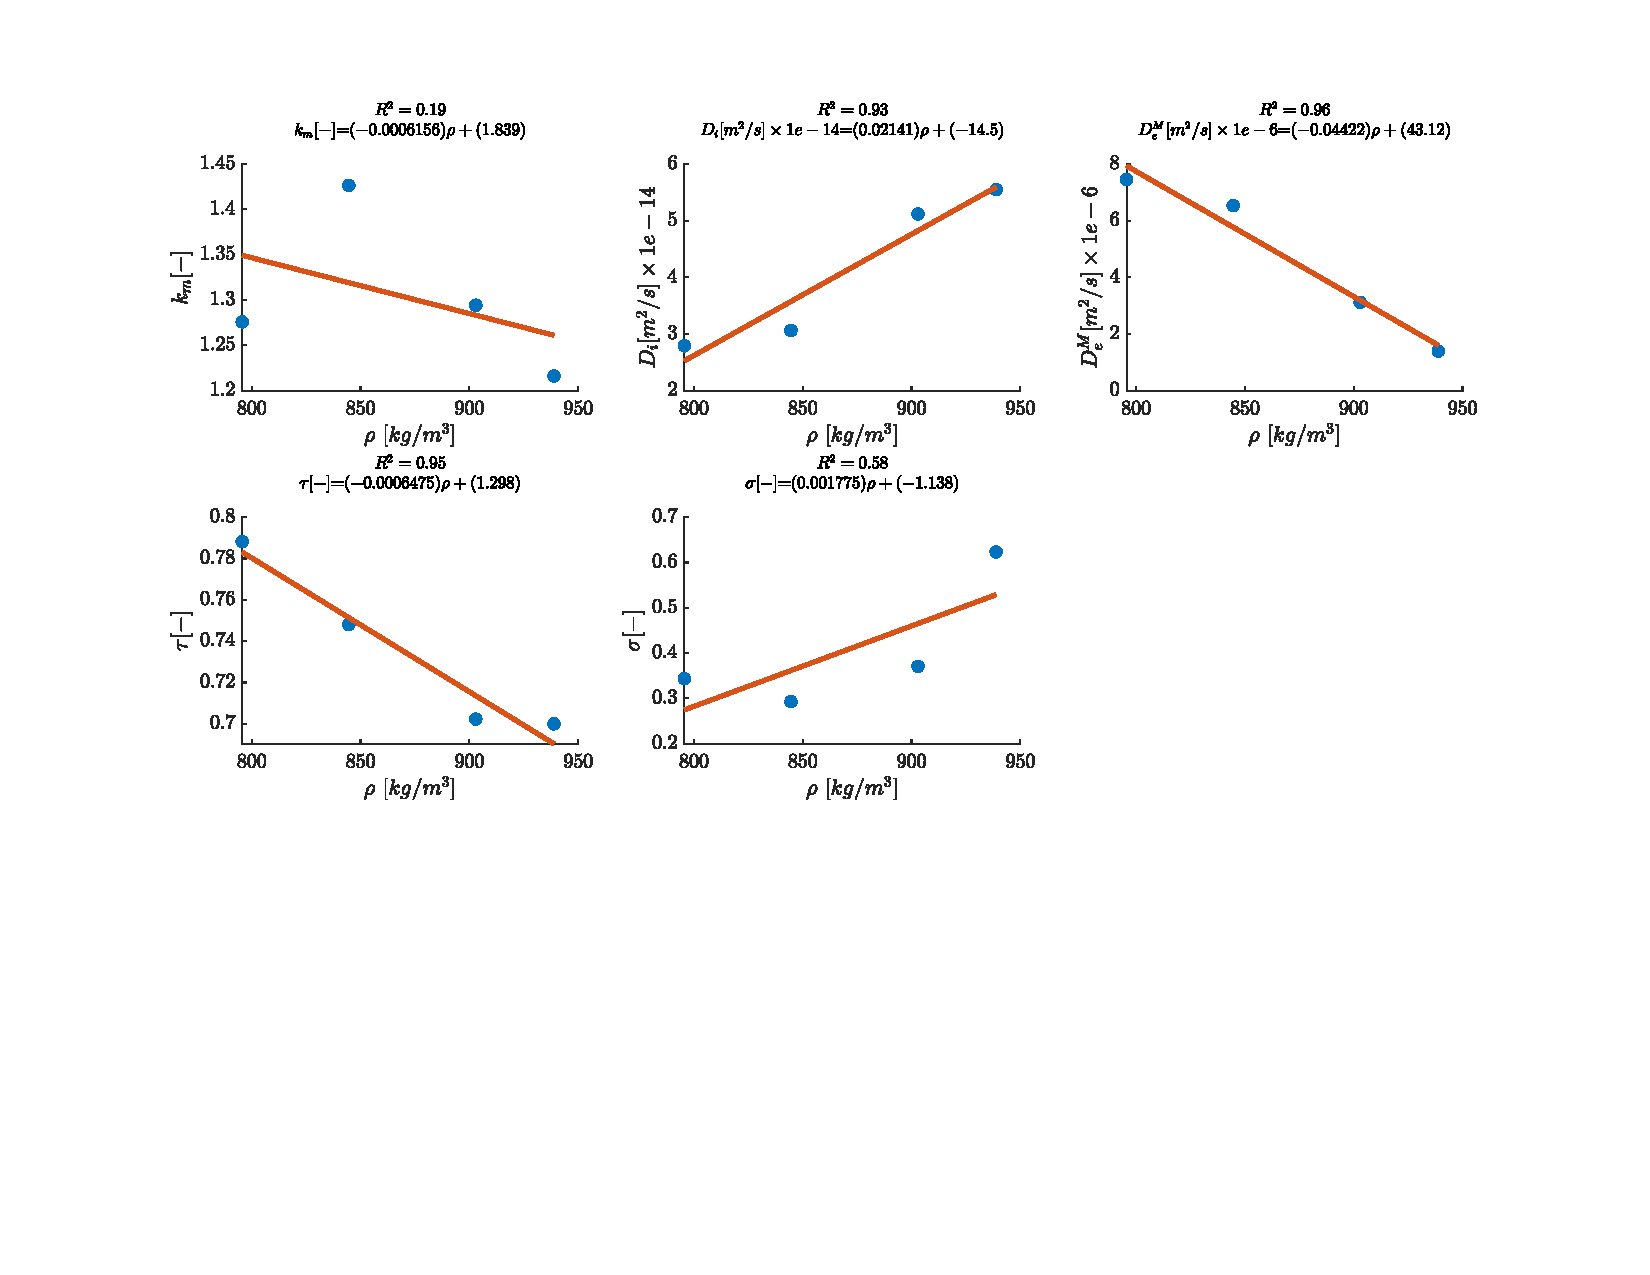
\includegraphics[trim = 1cm 2cm 2.5cm 1cm,clip,width=\textwidth]{/Results_estimation/Trend_Lines_order_1.pdf}
		\caption{First order polynomial regression of fitted parameters as a function of fluid density $\rho_f$}
	\end{subfigure}
	\hfill
	\begin{subfigure}[b]{0.85\textwidth}
		\centering
		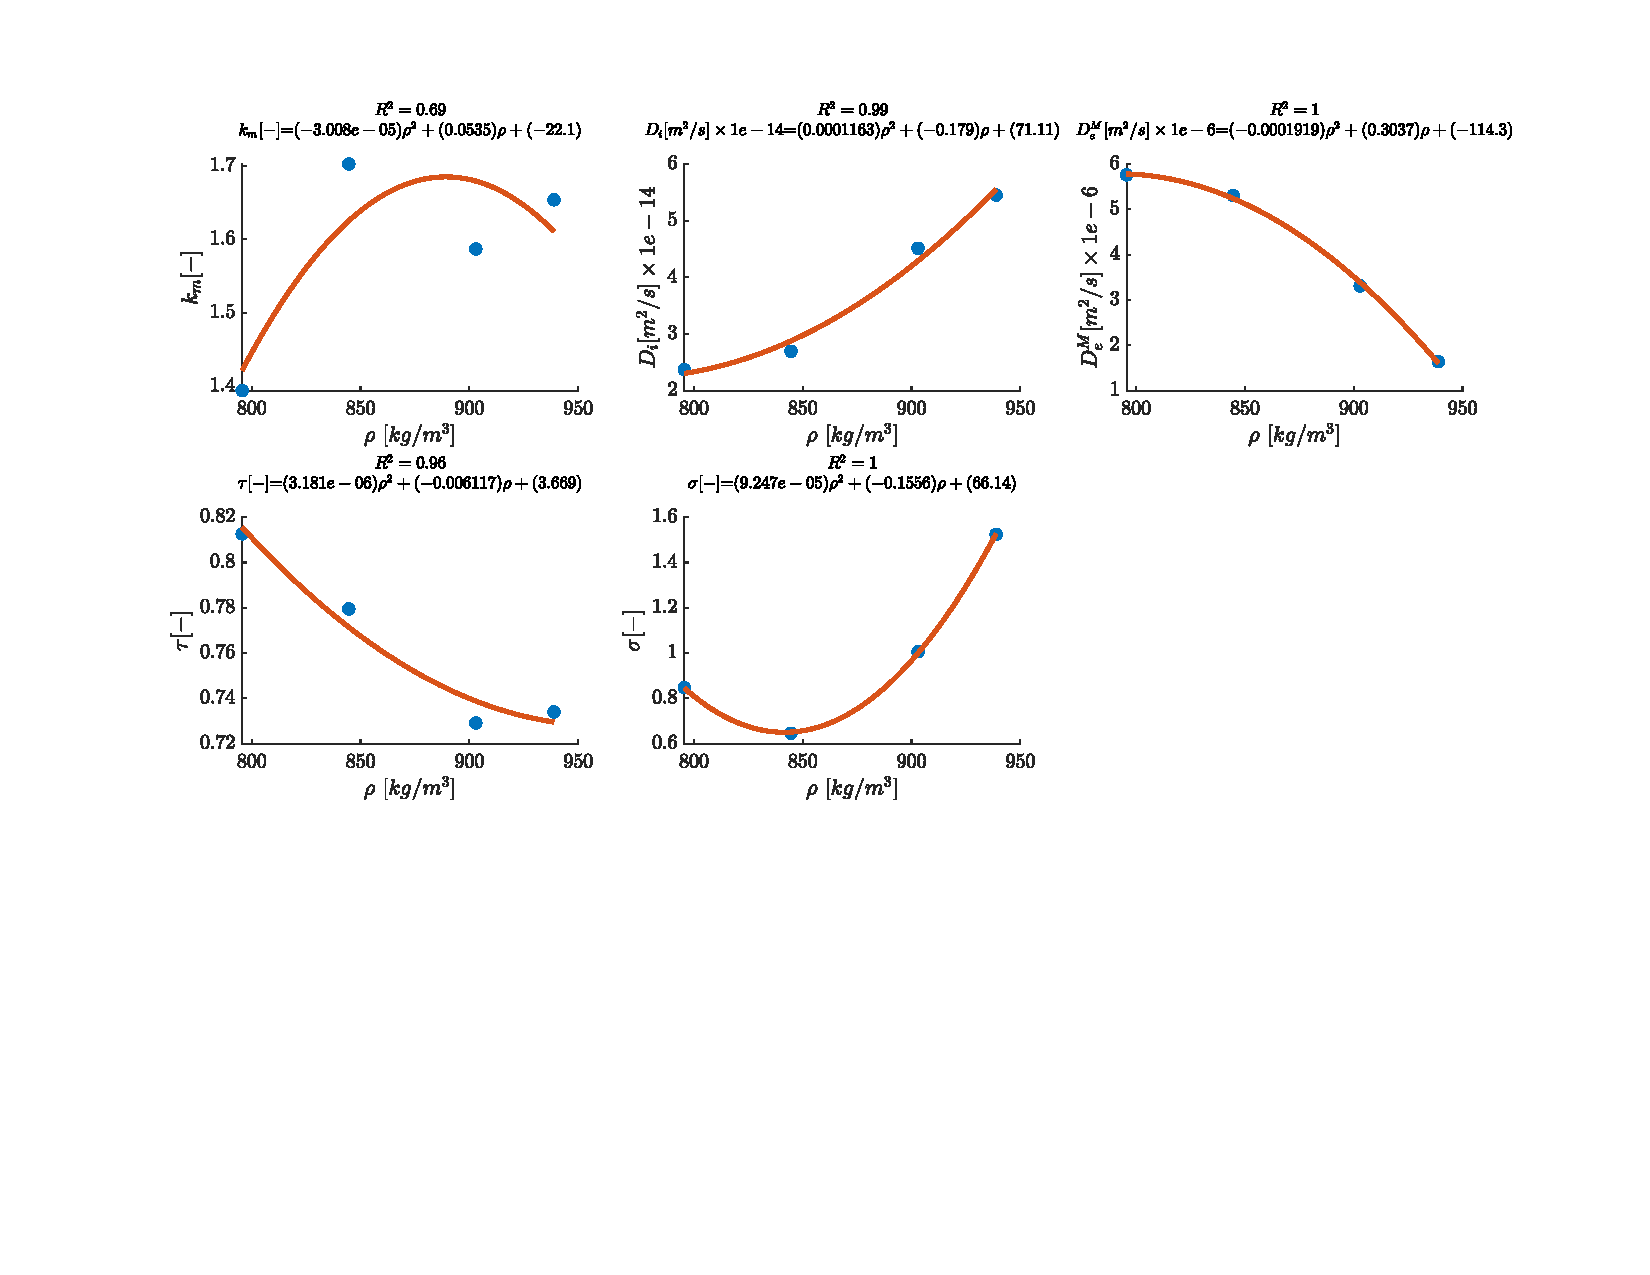
\includegraphics[trim = 1cm 2cm 2.5cm 1cm,clip,width=\textwidth]{/Results_estimation/Trend_Lines_order_2.pdf}
		\caption{Second order polynomial regression of fitted parameters as a function of fluid density $\rho_f$}
	\end{subfigure}
	\caption{Results of parameter fitting, with estimation of the initial state}
	\end{figure*}
	
	
\end{document}